\documentclass{article}

\usepackage[utf8]{inputenc}
\usepackage[T1]{fontenc}
\usepackage[french]{babel}
\usepackage{graphicx}

\newcommand{\bigo}{\mathcal{O}}

\title{Optimisation de l'évacuation en cas d'urgence}

\begin{document}

\maketitle

\section{Préambule}

Les objectifs de mon TIPE n'ont pas changé depuis la présentation du MCOT.
Nous avons gardé l'étude du bâtiment séparé de l'étude plus précise des salles.
Je me suis occupé de la deuxième partie avec un camarade, l'objectif est de
modéliser la sortie des agents, puis d'utiliser cette modélisation
pour améliorer les conditions d'évacuation en modifiant la salle et de
fournir à la modélisation du bâtiment des données précises sur le débit
de sortie des agents.

\section{Introduction}

Mon travail s'est surtout porté sur la modélisation de l'évacuation des
agents, en particulier sur le développement et l'implémentation
d'algorithme permettant aux agents de choisir le chemin à prendre, je
me concentrai donc seulement sur cette aspect du TIPE dans le rapport.
Le développement s'est fait de façon incrémentale en développant d'abord
des algorithmes simples pour après finir avec des algorithmes plus complexe
permettant dans certain cas une sortie efficace des agents.

\section{Corps Principal}

\subsection{Modalités d'action}

La première idée de modélisation fut de prendre en compte le voisinage de l'agent, l'agent ne prenant pas compte de ce qui est très loin de lui lors d'une situation
d'évacuation à l'exception de la sortie. Le choix de la direction à prendre pour
l'agent fut d'abord modéliser par la relation
entre les obstacles et des points placés autour de l'agent.

\begin{figure}[h]
  \centering
  \includegraphics[height=4cm]{img/testProximite.png}
  \caption{Un exemple de l'algorithme, seule les points non rouges sont considérés
    et le point le plus proche de la sortie -- le point bleu -- est utilisé}
\end{figure}

Puis nous avons utilisé
des lancers de rayons couplés à une dichotomie et une étude de distance entre les
obstacles pour prendre mieux en compte l'aspect continue de l'espace tout en gardant
une bonne efficacité.
Ces approches gloutonnes ne fonctionnant pas dans certains
cas particuliers, nous avons supposé la bonne connaissance de la salle par l'agent
pour dresser un champ vectorielle grâce à un parcours en largeurs depuis la sortie,
et enfin, pour atteindre un comportement plus réaliste pour les agents, nous avons
déterminé un champ scalaire grâce à un parcours en profondeur pour pouvoir en dériver
un gradient. La conformité des algorithmes à la réalité fut décidé à partir de
comparaison entre des mouvements réelles et le mouvement obtenue sur la simulation.

%Peut être parler des interpolations différentes utilisées

En plus de ces algorithmes permettant la sortie des agents, nous avons introduit
une vitesse variable en fonction de la densité surfacique d'agents à proximité
d'un agent permettant d'introduire un effet de groupe au mouvement des agents.

Le débit est extrait des temps de sortie des agents par une dérivation du nombre
de personnes sorties par rapport au temps.

\subsection{Restitution des résultats}

La modélisation du mouvement par placement
de points, ne permet pas la sortie de la totalité des agents et créé un mouvement
ne s'approchant pas du tout de la réalité.

%Image? Tracé du mouvements des agents?

Les différentes versions des algorithmes de lancé de rayons ont produit des
mouvement réalistes mais ont eu tendance à ralentir la simulation et ne permettais
pas la sortie d'une partie des agents dans des cas particulier

%Image? Tracé du mouvements (Équilibre stable dans des rangs proche de la sortie
%Évitement des obstacles polygonales, courbe d'efficacité / portions de la simulation
%prise par le choix de la direction

Les algorithmes utilisant un champ calculé au début de la simulation sont beaucoup
plus efficaces lors de la simulation que les autres algorithmes mais prennent en échange
un temps modeste en début de simulation pour construire le champ.

%Image sur le temps pris

L'algorithme utilisant un champ de vecteur permet une sortie de la totalité des
agents mais perd beaucoup de réalisme en poussant les agents à suivre un
quadrillage pour leur mouvement

%Image du champ

L'algorithme utilisant un champs de scalaire introduit bien le réalisme recherché
mais laisse des agents bloqué sur les coins d'obstacles rectangulaires proche
de la sortie

%Image du champ scalaire bilinéaire / bicubique et des champs de gradients associés
%Ainsi qu'une image témoignant du blocage sur les coins

L'introduction de la variation de la vitesse a permis d'introduire, comme voulus,
un mouvement plus réaliste: les agents bloqués ralentissent et ceux libres vont plus
vite que ceux bloqué

%Image témoignant de ceci

\subsection{Analyse-Exploitation-Discussion}

Le premier algorithme ne permet qu'un déplacement dans un nombre finis de directions
ce qui a induit le mouvement irréaliste, et les agents ne peuvent pas sortirent car
l'algorithme ne prend en compte que le voisinage de l'agent, ainsi l'agent peut se
retrouver dans un position stable où, lorsqu'il s'éloigne d'une zone avec obstacle,
il est susceptible d'y retourner. D'où le choix suivant du lancez de rayon qui
permet d'atteindre un nombre continue de directions possible -- modulo la borne
imposé par le stockage des flottants en Python -- et de prendre
mieux en compte la totalité du champ de vision d'un agent.

Les algorithmes de lancé de rayon sont une nette amélioration, l'utilisation
de la totalité du champ de vision des agents permet pour la plupart
d'éviter les obstacles et de sortir correctement, le choix non informé --
sans prendre en compte des positions antérieurs ou future -- laisse parfois les
agents immobile. Le ralentissement est du à un nombre $N$ de lancé de rayons
important lorsque que les obstacles sont proches de l'agent
\[
  N = \bigo\left(\frac{o}{p}\right) + \bigo\left(\ln\left(\frac{2 \pi - o}{p}\right)\right)
\]
où $o$ est la distance angulaire occupé par les obstacles et $p$ et la précision angulaire
du choix de la direction, ce ralentissement est aussi du à une implémentation
du lancé de rayon dans la librairie utilisé dont la complexité n'est pas optimale
$\bigo\left(k + \ln(n)\right)$ où $k$ est le nombre
d'obstacles sur le lancé de rayon et $n$ le nombre total d'obstacles, la complexité espéré
optimale
étant $\bigo(\ln(n))$ en utilisant la structure de donnée utilisée par la bibliothèque.

Le champ de vecteur est beaucoup plus efficace que les autres algorithmes, il est
prend moins de temps sur l'ensemble de la simulation car la construction
du champs se fait en $\bigo\left(\frac{surface\_salle}{p^2}\right)$ grâce à un parcours en largeur
et le choix du vecteur se fait en $\bigo(1)$ grâce à l'implémentation d'un hachage de
l'espace. Mais le parcours en largeur se faisant sur un quadrillage, le mouvement
des agents n'est pas réaliste.

L'algorithme utilisant le champ scalaire est légèrement plus lent que le champ
vectorielle car le calcul du gradient en une position donnée est plus lent,
il nécessite quelques produits matricielles pour interpoler les valeurs assignées
à différentes points, mais cette récupération est toujours en $\bigo(1)$. Le blocage des
agents sur les coins est surement du à des changements de direction trop rapide
dans le gradient et au fait que le volume des agents n'est pas pris en compte.

%L'introduction d'une procédure pour changer le champ scalaire au voisinage des obstacles
%pourrait permettre de régler ce problème, cette procédure pourrait être appliqué
%pour chaque agents pour prendre en compte son rayon qui varie d'un agent à un autre.

\section{Conclusion}

La modélisation du mouvement utilisé à finalement était celle de la dichotomie en évitant les
salles causant les immobilité des agents, grâce à cette modélisation nous avons vue que
le placement d'un obstacle en face de la sortie diminue le dé

\end{document}
